\begin{problem}[Nonlinear electric circuit]
  In previous exercises we have discussed electric circuits with elements that give
  rise to linear voltage--current dependence, see \lref{ex:elnet} and \lref{ex:Rspd}.
  The principles of nodal analysis were explained in these cases. 
  
  However, the electrical circuits encountered in practise usually feature elements
  with a \emph{non-linear} current-voltage characteristic. Then nodal analysis
  leads to non-linear systems of equations as was elaborated in \lref{ex:nlcirc}.
  Please note that transformation to frequency domain is not possible for
  non-linear circuits so that we will always study the direct current (DC)
  situation. 

  In this problem we deal with a very simple non-linear circuit element, a diode. The
  current through a diode as a function of the applied voltage can be modelled by the
  relationship
  $$I_{kj} = \alpha\Big(e^{\beta\frac{U_k-U_j}{U_T}}-1\Big),$$
  with suitable parameters $\alpha,\beta$ and the thermal voltage $U_{T}$. 

  Now we consider the circuit depicted in Fig.~\ref{fig:circ} and assume that all
  resistors have resistance $R=1$. 

    \begin{figure}
      \centering
      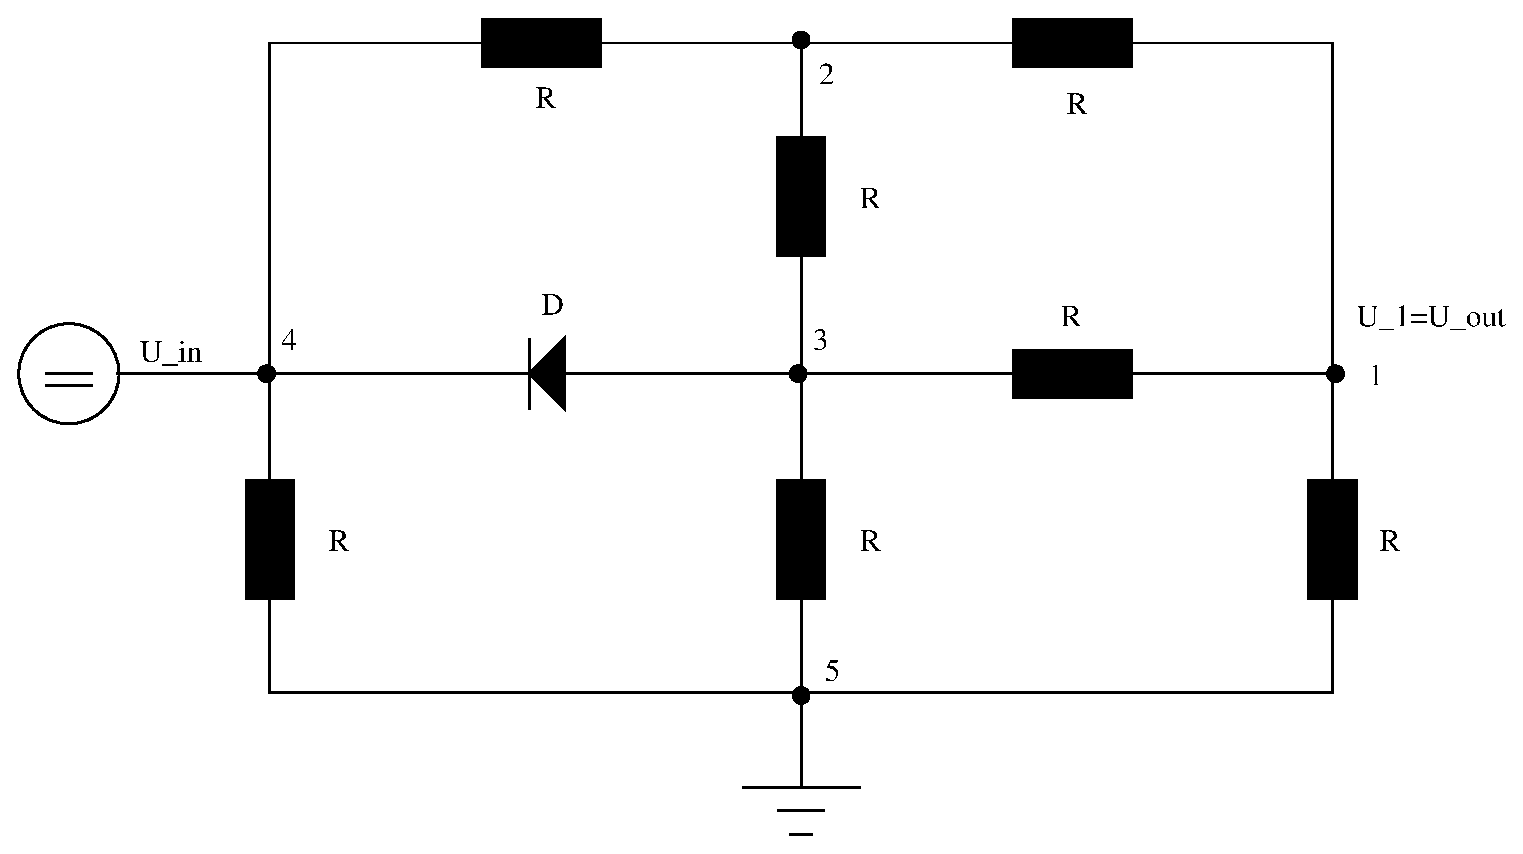
\includegraphics[scale=0.5]{\problems/ch_iterativenonlinear/PICTURES/circuit_diode.eps}
      \caption{non-linear circuit for Problem 1}
      \label{fig:circ}
    \end{figure}
    
  \begin{subproblem}[2]
    Carry out the nodal analysis of the electric circuit and
    derive the corresponding non-linear system of equations
    $\mathbf{F}(\mathbf{u})=\mathbf{0}$ for the voltages in nodes 1,2, and 3,
    \emph{cf.} \lref{eq:EMM}. Note that the voltages in nodes 4 and 5 are known
    (input voltage and ground voltage 0). 
    \begin{solution}
    We consider Kirchhoff's law $\sum\limits_{k,j} I_{kj} = 0$ for every node $k$. $I_{kj}$ contributes to the sum if node $j$
    is connected to node $k$ trough one element (R,C,L,D).
    
    \begin{itemize}
        \item[(1)] $3U_1 - 0 - U_2 - U_3=0$
        \item[(2)] $3U_2 - U_1 - U_3 - U=0$
        \item[(3)] $3U_3 - 0 - U_1 - U_2+ \alpha\Bigg(e^{\beta\Big(\frac{U_3-U}{U_T} \Big)}-1\Bigg)=0 $
    \end{itemize}
    
    Thus the nonlinear system of equations reads
    $$\mathbf{F}(\mathbf{u})=\left(\begin{array}{l}3U_1-U_2-U_3 \\ 3U_2-U_1-U_3-U \\ 
      3U_3-U_1-U_2 +\alpha e^{-\frac{\beta}{U_T}U}\cdot e^{\frac{\beta}{U_T}U_3} -\alpha \end{array}\right)=
      \left(\begin{array}{c} 0 \\0\\ 0\end{array}\right) \qquad \text{for } \mathbf{u}=\left(\begin{array}{c}U_1 \\ U_2 \\ U_3 \end{array}\right). $$
    \end{solution}
  \end{subproblem}

  \begin{subproblem}[3]
    Write an \Eigen{} function 
    \begin{lstlisting}
    void circuit(const double & alpha, const double & beta, const VectorXd & Uin, VectorXd & Uout)
    \end{lstlisting}
    that computes the output voltages \texttt{Uout} (at node 1 in Fig.~\ref{fig:circ}) for a
    \emph{sorted} vector of input voltages \texttt{Uin} (at node 4) for a thermal voltage $U_T=0.5$. The
    parameters \texttt{alpha}, \texttt{beta} pass the (non-dimensional) diode
    parameters. 

    Use Newton's method to solve $\mathbf{F}(\mathbf{u})=\mathbf{0}$ with
    a tolerance of $\tau=10^{-6}$.
      \begin{solution}
      An iteration of the multivariate Newton method is:
    $$ \mathbf{u}^{(k+1)} = \mathbf{u}^{(k)} - \big(D\mathbf{F}(\mathbf{u}^{(k)}\big)^{-1}\mathbf{F}(\mathbf{u}^{(k)}) $$
    The components of the Jacobian $D\mathbf{F}$ are defined as $D\mathbf{F}(\mathbf{u})_{ij}:=\frac{\partial F_i(\mathbf{u})}{\partial u_j}$. 
    For the function obtained in a) we get
    $$ D\mathbf{F}(\mathbf{u})=\mathbf{J}=\left(\begin{array}{rrl}3 & -1 & -1 \\ -1 & 3 & -1 \\ -1 & -1 & 3+ \frac{\alpha\beta}{U_T}e^{\beta\frac{U_3-U}{U_T}} \end{array}\right).$$
     For the implementation in Eigen see file \texttt{nonlinear\_circuit.cpp}.
            \end{solution}
  \end{subproblem}
      \begin{subproblem}[2]
      We are interested in the nonlinear effects introduced by the diode. Calculate
      $U_{\text{out}}=U_{\text{out}}(U_{\text{in}})$ as a function of the variable
      input voltage $U_{\text{in}}\in[0,20]$ (for non-dimensional parameters
      $\alpha=8$, $\beta=1$ and for a thermal voltage $U_T=0.5$) and infer the nonlinear effects from the results.
       \begin{solution}
 The nonlinear effects can be observed by calculating the differences between the solutions $U_{\text{out}}$, see file \texttt{nonlinear\_circuit.cpp}.
       \end{solution}
    \end{subproblem}
  \end{problem}